\section{Introducción}
En este trabajo se aborda una solución para el problema de satisfacibilidad. Este problema trata de buscar si una fórmula proposicional es o no satisfacible. Para ello, hay que encontrar una asignación para cada una de las variables que aparecen en cada clausula de la fórmula y comprobar que dicha asignación hace verdadera cada una de las clausulas que componen dicha fórmula.\\
El algoritmo que se ha usado se llama \textit{Survey Propagation}, diseñado por A. Braunstein, M. Mezard, R. Zecchina. \\\\
Una fórmula proposicional está compuesta por un conjunto de clausulas y cada clausula está formada por un conjunto variables booleanas conectadas con unos operadores. Un ejemplo de una formula de 2 clausulas y 3 variables seria: $x \lor (y \land z)$.\\\\
En este trabajo se ha usado estas formulas en su \textbf{Forma Normal Conjuntiva} (CNF en inglés).
Una fórmula estará en forma normal conjuntiva si corresponde a una conjunción de clausulas, donde cada clausula es una disyunción de literales. Un literal es La forma normal conjuntiva de la formula anterior es $(x \lor y)\land (x \lor z)$.\\\\
Si tenemos la fórmula en forma normal conjuntiva, el objetivo es buscar aquella asignación que satisfaga cada una de las clausulas que componen la fórmula. Una interpretación que satisface la formula anterior seria:
\begin{itemize}
	\item $x=1$
	\item $y=0$
	\item $z=0$
\end{itemize}
Si nos fijamos, en la formula anterior con que la variable $x$ sea verdadera sería suficiente para que la fórmula sea satisfacible.\\\\
El problema de satisfacibilidad booleana es un problema muy importante en el campo de la informática. Fue el primer problema que se demostró que era NP-completo. Fué demostrado por Stephen Cook en 1971.\\
En este caso, tenemos 3 variables y tenemos un total de $2^3 = 8$ asignaciones distintas. Aquí podemos ver que este problema va a tener un espacio de búsqueda que va a crecer de forma exponencial a medida que se incrementa el número de variables. 
Dentro del mundo de la computación, este problema pertenece a la clase de complejidad NP-completo, es decir, no conocemos un algoritmo que sea capaz de resolver este problema en un tiempo polinomial.\\\\
Hay un gran interés en encontrar una solución a este problema, ya que al ser NP-completo, el resto de problemas pertenecientes a la clase NP se pueden reducir (realizar una conversión para adaptar el problema NP al problema SAT) a SAT, y encontrando una solución a SAT se podría usar dicha solución para resolver cualquier problema dentro de la clase NP.\\\\
El algoritmo \textit{Survey Propagation} es un algoritmo aproximado, es decir, si hay una formula que es satisfacible \textbf{puede} (o no) encontrar una interpretación que la satisfaga.
Estos algoritmos son de interés debido a que suelen ser mejores en tiempo a la hora de resolver problemas más grandes debido a que no son tan costosos a la hora de ejecutarlos como algoritmos clásicos (branch \& bound, búsqueda en profundidad, etc).\\\\
En este trabajo se afronta también la integración con un algoritmo completo llamado Glucose. Esta integración se explicará de una forma más detallada en secciones siguientes, pero como resumen, ambos algoritmos tienen una fase en la que se selecciona una variable de la formula y se asigna siguiendo un criterio. Lo que se ha hecho es usar el criterio de \textit{Survey propagation} para seleccionar una variable y su asignación en el algoritmo Glucose.
\pagebreak
\section{Fundamentos matemáticos}
En el álgebra de Boole las variables tienen dos estados: verdadero o falso y se definen los siguientes operadores:
\begin{enumerate}[1.]
	\item \textbf{Complementario:} $\neg$ Este operador unario nos convierte una variable al estado contrario (de falso a verdadero y de verdadero a falso).
	\item \textbf{Disyunción:} $\lor$ Este operador binario devuelve verdadero si una de los dos variables está en el estado verdadero.
	\item \textbf{Conjunción:} $\land$ Este operador binario devuelve verdadero solo cuando ambas variables sean verdaderas.
\end{enumerate}
\subsection{Representación Factor Graph}
Este algoritmo hace uso de una representación en forma de grafo bipartito para resolver el problema. Esta representación se caracteriza por lo siguiente:
\begin{enumerate}
	\item Tenemos dos tipos de nodos:
	\begin{itemize}
		\item \textbf{Nodo variable.}
		\item \textbf{Nodo clausula.}
	\end{itemize}
	\item Tenemos dos tipos de aristas:
	\begin{itemize}
		\item \textbf{Positiva.}
		\item \textbf{Negativa.}
	\end{itemize}
\end{enumerate}
Por cada variable que aparezca en la formula habrá un nodo variable. De igual manera ocurre con las clausulas, por cada clausula tendremos su correspondiente nodo clausula en el grafo. 
Si una variable $x$ aparece en una clausula $i$ habrá una arista positiva si dicha variable aparece no negada y será negativa cuando dicha variable esté negada dentro de la clausula.\\\\
A continuación se muestra una representación gráfica usando esta representación de la siguiente fórmula: \[F = (x_1 \lor\neg x_3) \land (\neg x_1 \lor x_2 \lor x_4) \land (\neg x_3 \lor x_5) \land (\neg x_3 \lor \neg x_4 \lor x_5) \land (\neg x_2 \lor x_4 \lor x_6) \land (x_5)\]
\pagebreak
\begin{figure}[!htbp]
	\centering
	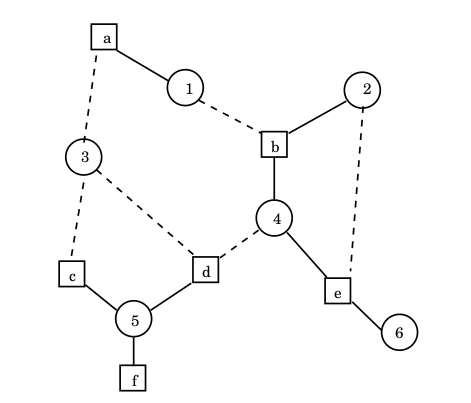
\includegraphics[scale=0.5]{img/fg}
	\label{img:fg1}
	\caption{Representación en factor graph de una fórmula.}
\end{figure}\\
En esta figura cada clausula se representa con una letra y las variables con los números que aparecen en los sub-índices de las variables. Por ejemplo si nos fijamos en la primera clausula, vemos que la variable $x_3$ aparece negada y la variable $x_1$ aparece sin negar. En el grafo, vemos como el nodo clausula $a$ esta conectado con una linea continua (no negada) al nodo variable $1$ y conectado con una linea discontinua (negada) al nodo variable $3$. \\\\
Usando esta representación, se van a definir unos conjuntos que se usaran en el algoritmo: 
\begin{itemize}
	\item
\end{itemize}